%% Copyright (c) 2015-2019, RTE (http://www.rte-france.com)
%% See AUTHORS.txt
%% All rights reserved.
%% This Source Code Form is subject to the terms of the Mozilla Public
%% License, v. 2.0. If a copy of the MPL was not distributed with this
%% file, you can obtain one at http://mozilla.org/MPL/2.0/.
%% SPDX-License-Identifier: MPL-2.0
%%
%% This file is part of Dynawo, an hybrid C++/Modelica open source time domain simulation tool for power systems.

\documentclass[a4paper, 12pt]{report}

%% Except where otherwise noted, content in this documentation is Copyright (c)
%% 2015-2019, RTE (http://www.rte-france.com) and licensed under a
%% CC-BY-4.0 (https://creativecommons.org/licenses/by/4.0/)
%% license. All rights reserved.

% Latin Modern fam­ily of fonts
\usepackage{lmodern}

\usepackage[english]{babel}

% specify encoding
\usepackage[utf8]{inputenc} % input
\usepackage[T1]{fontenc} % output

% Document structure setup
\usepackage{titlesec} % To change chapter format
\setcounter{tocdepth}{3} % Add subsubsection in Content
\setcounter{secnumdepth}{3} % Add numbering for subsubsection
\setlength{\parindent}{0pt} % No paragraph indentation

% Change title format for chapter
\titleformat{\chapter}{\Huge\bf}{\thechapter}{20pt}{\Huge\bf}

% To add links on page number in Content and hide red rectangle on links
\usepackage[hidelinks, linktoc=all]{hyperref}
\usepackage[nottoc]{tocbibind}  % To add biblio in table of content
\usepackage{textcomp} % For single quote
\usepackage{url} % Allow linebreaks in \url command
\usepackage{listings} % To add code samples

% Default listings parameters
\lstset
{
  aboveskip={1\baselineskip}, % a bit of space above
  backgroundcolor=\color{shadecolor}, % choose the background color
  basicstyle={\ttfamily\footnotesize}, % use font and smaller size \small \footnotesize
  breakatwhitespace=true, % sets if automatic breaks should only happen at whitespace
  breaklines=true, % sets automatic line breaking
  columns=fixed, % nice spacing -> fixed / flexible
  mathescape=false, % escape to latex false
  numbers=left, % where to put the line-numbers
  numberstyle=\tiny\color{gray}, % the style that is used for the line-numbers
  showstringspaces=false, % do not emphasize spaces in strings
  tabsize=4, % number of spaces of a TAB
  texcl=false, % activates or deactivates LaTeX comment lines
  upquote=true % upright quotes
}

% Avoid numbering starting at each chapter for figures
\usepackage{chngcntr}
\counterwithout{figure}{chapter}

\usepackage{tikz} % macro pack­age for cre­at­ing graph­ics
\usepackage{pgfplots} % draws func­tion plots (based on pgf/tikz)

\usepackage{algorithm} % Add algorithms
\usepackage[noend]{algpseudocode} %  all end ... lines are omitted in algos

\usepackage{amsmath} % Add math­e­mat­i­cal fea­tures
\usepackage{schemabloc} % Add block diagram library (french one)

\usepackage{adjustbox} % Add box for flowchart

\usepackage{booktabs} % for toprule and midrule in tables

\usepackage{tabularx}

\usepackage[nolist]{acronym} % don’t write the list of acronyms.
% Acronyms list
\begin{acronym}
\acro{BDF}{Backward Differentiation Formula}
\acro{BE}{Backward Euler}
\acro{DAE}{Differential Algebraic Equations}
\acro{IDA}{Implicit Differential-Algebraic solver}
\acro{LLNL}{Lawrence Livermore National Lab}
\acro{KINSOL}{Krylov Inexact Newton SOLver}
\acro{NR}{Newton-Raphson}
\acro{PLL}{Phase-Locked Loop}
\acro{SVC}{Static Var Compensator}
\acro{SUNDIALS}{SUite of Nonlinear and DIfferential/ALgebraic equation Solvers}
\acro{WECC}{Western Electricity Coordinating Council}
\end{acronym}

% Syntax highlight
%% Except where otherwise noted, content in this documentation is Copyright (c)
%% 2015-2019, RTE (http://www.rte-france.com) and licensed under a
%% CC-BY-4.0 (https://creativecommons.org/licenses/by/4.0/)
%% license. All rights reserved.

\usepackage{color}

\definecolor{blue}{rgb}{0,0,1}
\definecolor{lightblue}{rgb}{.3,.5,1}
\definecolor{darkblue}{rgb}{0,0,.4}
\definecolor{red}{rgb}{1,0,0}
\definecolor{darkred}{rgb}{.56,0,0}
\definecolor{pink}{rgb}{.933,0,.933}
\definecolor{purple}{rgb}{0.58,0,0.82}
\definecolor{green}{rgb}{0.133,0.545,0.133}
\definecolor{darkgreen}{rgb}{0,.4,0}
\definecolor{gray}{rgb}{.3,.3,.3}
\definecolor{darkgray}{rgb}{.2,.2,.2}
\definecolor{shadecolor}{gray}{0.925}

% **********************************************************************************
% Syntax : Bash (bash)
% **********************************************************************************

\lstdefinelanguage{bash}
{
  keywordstyle=\color{blue},
  morekeywords={
    cd,
    export,
    source},
  numbers=none,
  deletekeywords={jobs}
}

% **********************************************************************************
% Syntax : XML
% **********************************************************************************

\lstdefinelanguage{XML}
{
  morestring=[s][\color{purple}]{"}{"},
  morecomment=[s][\color{green}]{<?}{?>},
  morecomment=[s][\color{green}]{<!--}{-->},
  stringstyle=\color{black},
  identifierstyle=\color{blue},
  keywordstyle=\color{red},
  morekeywords={
    xmlns,
    xsi,
    noNamespaceSchemaLocation,
    type,
    source,
    target,
    version,
    tool,
    transRef,
    roleRef,
    objective,
    eventually}
}

% **********************************************************************************
% Syntax : Modelica (modelica)
% **********************************************************************************
\lstdefinelanguage{Modelica}{
  alsoletter={...},
  morekeywords=[1]{ % types
      Boolean,
      Integer,
      Real},
  keywordstyle=[1]\color{red},
  morekeywords=[2]{ % keywords
    algorithm,
    and,
    annotation,
    assert,
    block,
    class,
    connector,
    constant,
    discrete,
    else,
    elseif,
    elsewhen,
    end,
    equation,
    exit,
    extends,
    external,
    false,
    final,
    flow,
    for,
    function,
    if,
    in,
    inner,
    input,
    import,
    loop,
    model,
    nondiscrete,
    not,
    or,
    outer,
    output,
    package,
    parameter,
    public,
    protected,
    record,
    redeclare,
    replaceable,
    return,
    size,
    terminate,
    then,
    true,
    type,
    when,
    while},
  keywordstyle=[2]\color{darkred},
  morekeywords=[3]{ % functions
    abs,
    acos,
    asin,
    atan,
    atan2,
    Complex,
    connect,
    conj,
    cos,
    cosh,
    cross,
    der,
    edge,
    exp,
    fromPolar,
    imag,
    noEvent,
    pre,
    sign,
    sin,
    sinh,
    sqrt,
    tan,
    tanh},
  keywordstyle=[3]\color{blue},
  morecomment=[l][\color{green}]{//}, % comments
  morecomment=[s][\color{green}]{/*}{*/}, % comments
  morestring=[b][\color{pink}]{'}, % strings
  morestring=[b][\color{pink}]{"}, % strings
}


\usepackage{xspace} % Define typography
\usepackage{dirtree}
\newcommand{\Dynawo}[0]{Dyna$\omega$o\xspace}


\begin{document}

\chapter{Impact of the excitation control on a synchronous generator transient stability}

This test case is inspired by example 13.2 of Kundur "Power System Stability and Control" book.

% Generic description of the non regression test
% List of scenarios
\section{Test case description}

This test case compares the behavior of a synchronous machine subject to a 3-phase fault with three different excitation controls:
\begin{itemize}
\item a set-point;
\item a proportional voltage regulator;
\item a proportional voltage regulator with a PSS function;
\end{itemize}
To do so, a simple Synchronous Machine - Infinite Bus (SMIB) system is used. It consists of a single machine connected to the infinite bus through two parallel lines and a transformer as presented in Figure 1.

\begin{figure}[H]
\centering
\def\factor{0.4}
\begin{tikzpicture}[every node/.style={inner sep=0,outer sep=0}]
% Infinite bus
\path (0,0)  pic[scale=0.2,local bounding box=bus] {infinite bus};
%% Transfo
\path (5,0) pic[scale=0.2,local bounding box=transfo] {transfo};
% Generator
\path (8,0) pic[scale=0.2,local bounding box=gen] {generator};
% Line 1
\draw ([yshift=0.25cm]bus.east) -- ([yshift=0.25cm]transfo.west);
% Line 1
\draw ([yshift=-0.25cm]bus.east) -- ([yshift=-0.25cm]transfo.west);
% Bus inf
\draw (bus.east) ++ (0,0.5) --++ (0,-1);
% Bus tfo 1
\draw (transfo.west) ++ (0,0.5) node (bustop) {} --++ (0,-1) node (busbottom) {};
% Bus tfo 2
\draw (transfo.east) ++ (0,0.3) node (bustop) {} --++ (0,-0.6) node (busbottom) {};
% Transfo-Generator connection
\draw (transfo.east) -- (gen.west);
\end{tikzpicture}
\caption{SMIB system representation}
\label{circuit-1}
\end{figure}

The SMIB system is a well-known test case in the power system community. It is very often used to illustrate the transient or the small-signal stability of a synchronous machine. It is also used to demonstrate the behavior of a new regulation, such as a speed governor, a voltage regulation or a power-system stabilizer.

\subsection{Initial Conditions}

The infinite bus base voltage is 400 kV and the synchronous machine base voltage is 24 kV. \\

The generator is a 2220 MVA equivalent for four 555 MVA generators.\\

The lines and transformer parameters in per unit on 100 MVA base are:
\begin{center}
\begin{tabular}{l|l|l}
   $R_1=0$ & $R_2=0$ & $R_{Tfo}=0$ \\
   $X_1=0.022522$ & $X_2=0.04189$ & $X_{Tfo}=0.00675$ \\
\end{tabular}
\end{center}

The reference angle for the load flow is set at the infinite bus, and the voltage amplitude at the machine terminal is set to 1. \\

The load flow results in per unit on 100 MVA base are:
\begin{center}
\begin{tabular}{l|l|l}
   $U_{Inf}=0.90081$ & $U_{SM}=1$ & $P_{SM}=19.98$ \\
   $\Theta_{Inf}=0rad$ & $\Theta_{SM}=0.49445rad$ & $Q_{SM}=9.68$ \\
\end{tabular}
\end{center}

\subsection{Models}

The equivalent generator parameters are given in per unit on 2220 MVA - 24 kV (no transformer included, no saturation):
\begin{center}
\begin{tabular}{l|l|l|l}
   $R_a=0.003$ & $X_l=0.15$ & $H=3.5$ & $D=0$ \\
   $X_d=1.81$ & $T'_d0=8s$ & $X_q=1.76$ & $T'_q0=1s$ \\
   $X'_d=0.30$ & $T''_d0=0.03s$ & $X'_q=0.65$ & $T''_q0=0.07s$ \\
   $X''_d=0.23$ & & $X''_q=0.25$ &  \\
\end{tabular}
\end{center}

The system reference frequency omegaRef is set to 1.\\
The machine is under constant mechanical power. \\
The voltage regulator is as follows:
\begin{figure}[H]
\centering
\begin{tikzpicture}
\sbEntree{E}
\sbBloc[3]{Transducer}{$\dfrac{1}{1+s\cdot T_R}$}{E}
\sbRelier[$U_S$]{E}{Transducer}
\sbCompSum[5]{errAVR}{Transducer}{+}{+}{-}{}
\sbRelier{Transducer}{errAVR}
\sbDecaleNoeudy[-4]{errAVR}{Uc}
\sbRelier[$U_C$]{Uc}{errAVR}
\sbBloc{Exciter}{$K_A$}{errAVR}
\sbRelier{errAVR}{Exciter}
\sbBlocL{Limiter}{\tikz {\draw (-0.4,-0.4) -- (0,-0.4);\draw (0,-0.4) -- (0,0.4); \draw (0,0.4) -- (0.4,0.4); }}{Exciter}
\sbSortie[5]{S}{Limiter}
\sbRelier[$Efd$]{Limiter}{S}
\sbDecaleNoeudy[4]{errAVR}{VPSS}
\sbRelier[$V_{PSS}$]{VPSS}{errAVR}
\end{tikzpicture}
\caption{Voltage regulator}
\end{figure}

The signal $V_{PSS}$ is set to zero if no PSS is used.


The voltage regulator parameters are:
\begin{center}
\begin{tabular}{l|l}
   $K_A=200$ & $Efd_{Max}=7$  \\
   $T_R=0.015s$ & $Efd_{Min}=-6.4$   \\
\end{tabular}
\end{center}

A PSS is used in one of the test, in order to see its influence on the synchronous machine transient stability. Its structure is as follows:
\begin{figure}[H]
\centering
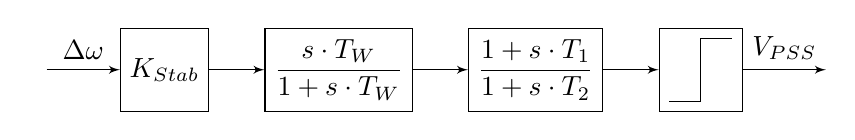
\begin{tikzpicture}
\sbEntree{E}
\sbBloc[3]{Gain}{$K_{Stab}$}{E}
\sbRelier[$\Delta \omega$]{E}{Gain}
\sbBloc{Washout}{$\dfrac{s\cdot T_W}{1+s\cdot T_W}$}{Gain}
\sbRelier{Gain}{Washout}
\sbBloc{PhaseCompensation}{$\dfrac{1+s\cdot T_1}{1+s\cdot T_2}$}{Washout}
\sbRelier{Washout}{PhaseCompensation}
\sbBlocL{LimiterPSS}{\tikz {\draw (-0.4,-0.4) -- (0,-0.4);\draw (0,-0.4) -- (0,0.4); \draw (0,0.4) -- (0.4,0.4); }}{PhaseCompensation}
\sbSortie[3]{S}{LimiterPSS}
\sbRelier[$V_{PSS}$]{LimiterPSS}{S}
\end{tikzpicture}
\caption{Power System Stabilizer structure}
\end{figure}

The power system stabilizer parameters are:
\begin{center}
\begin{tabular}{l|l|l}
   $K_{Stab}=9.5$ & $T_1=0.154s$ & $Vs_{Max}=0.2$  \\
   $T_W=1.41s$ & $T_2=0.033s$ & $Vs_{Min}=-0.2$   \\
\end{tabular}
\end{center}

\subsection{Scenario}
The simulated scenario is :
\begin{itemize}
\item at $t=1s$: a 0.07s three-phase fault at the transformer high voltage terminal;
\item at $t=1.07s$: the opening of line 2;
\end{itemize}

\subsection{Solver}
The solver used is the variable time step solver IDA with the following parameters:
\begin{itemize}
\item $Order$=2;
\item $Accuracy_{Rel}$=10e-4;
\item $Accuracy_{Abs}$=10e-4;
\end{itemize}

\section{Results}

The results of the simulations performed with the different excitation controls are presented bellow. Here are the different observations:
\begin{itemize}
\item with a constant excitation voltage, the system remains stable but the level of the oscillations damping is low;
\item with the proportional voltage regulator, the system loses synchronism in the third swing. The regulator's gain is very high and the control acts to fast, it destabilizes the system;
\item with the proportional voltage including a PSS function, the system remains stable and the oscillations are very well damped. We see here the positive impact of the PSS on the machine's stability;
\end{itemize}

These results match the results obtained in the example 13 of the "Power System Stability and Control" book of P.Kundur.

\begin{figure}[H]
  \caption{Rotor angle (deg)}
  \begin{tikzpicture}
    \begin{axis} [ymin = 0, ymax = 3.14, legend style={at={(0.5,-0.1)},anchor=north}]
        \addplot[color=red!50]
        table[x=time, y=SM_gen_theta]
        {../reference/outputs_AVR_SetPoint/curves/curves.csv};
        \addplot[color=blue!50]
        table[x=time, y=SM_gen_theta]
        {../reference/outputs_AVR_NoPSS/curves/curves.csv};
        \addplot[color=green!50]
        table[x=time, y=SM_gen_theta]
        {../reference/outputs_AVR_PSS/curves/curves.csv};
        \legend{$SetPoint$, $AVRNoPSS$, $AVRWithPSS$}
    \end{axis}
  \end{tikzpicture}
\end{figure}

\begin{figure}[H]
  \caption{Stator voltage (p.u)}
  \begin{tikzpicture}
    \begin{axis}[legend style={at={(0.5,-0.1)},anchor=north}]
        \addplot[color=red!50]
        table[x=time, y=SM_gen_UPu]
        {../reference/outputs_AVR_SetPoint/curves/curves.csv};
        \addplot[color=blue!50]
        table[x=time, y=SM_gen_UPu]
        {../reference/outputs_AVR_NoPSS/curves/curves.csv};
        \addplot[color=green!50]
        table[x=time, y=SM_gen_UPu]
        {../reference/outputs_AVR_PSS/curves/curves.csv};
        \legend{$SetPoint$, $AVRNoPSS$, $AVRWithPSS$}
    \end{axis}
  \end{tikzpicture}
\end{figure}

\begin{figure}[H]
  \caption{Active power (p.u)}
  \begin{tikzpicture}
    \begin{axis} [ymin = 0, legend style={at={(0.5,-0.1)},anchor=north}]
        \addplot[color=red!50]
        table[x=time, y=SM_gen_PGenPu]
        {../reference/outputs_AVR_SetPoint/curves/curves.csv};
        \addplot[color=blue!50]
        table[x=time, y=SM_gen_PGenPu]
        {../reference/outputs_AVR_NoPSS/curves/curves.csv};
        \addplot[color=green!50]
        table[x=time, y=SM_gen_PGenPu]
        {../reference/outputs_AVR_PSS/curves/curves.csv};
        \legend{$SetPoint$, $AVRNoPSS$, $AVRWithPSS$}
    \end{axis}
  \end{tikzpicture}
\end{figure}

\end{document}
